\documentclass[10pt]{article}
\usepackage[a4paper, tmargin=0.75in, lmargin=0.80in, rmargin=0.80in, bmargin=1in]{geometry}
\usepackage{hyperref}
%\usepackage{multicol}
\hypersetup{
    colorlinks=true,
    linkcolor=black,
    filecolor=magenta,      
    urlcolor=blue,
    citecolor=black,
}
%\usepackage[numbers,sort&compress]{natbib} % for a numerical citation list
\usepackage{natbib} % to cite references by surname and year
\usepackage{graphicx}
\usepackage{fancyvrb}
\usepackage{amsmath}
\usepackage{braket}
\pagestyle{empty}


%%%%%%%%%%%%%%%%%%%%%%%%%%%%%%%%%%%%%%%%%%%%%%%%%%
%%%%%%%%%%%%%%%%%%%%%%%%%%%%%%%%%%%%%%%%%%%%%%%%%%
%%%%%%%%%%%%%%%%%%%%%%%%%%%%%%%%%%%%%%%%%%%%%%%%%%
%%%%%%%%%%%%%%%%%%%%%%%%%%%%%%%%%%%%%%%%%%%%%%%%%%
% ENTER SOME IMPORTANT INFORMATION
%%%%%%%%%%%%%%%%%%%%%%%%%%%%%%%%%%%%%%%%%%%%%%%%%%
%%%%%%%%%%%%%%%%%%%%%%%%%%%%%%%%%%%%%%%%%%%%%%%%%%
%%%%%%%%%%%%%%%%%%%%%%%%%%%%%%%%%%%%%%%%%%%%%%%%%%
%%%%%%%%%%%%%%%%%%%%%%%%%%%%%%%%%%%%%%%%%%%%%%%%%%
\newcommand{\studentname}{Kartheek Tammana, Kushagra Gupta, Rishit Devalacheruvu}
\newcommand{\studentnumber}{cs21btech11028, cs21btech11033, cs21btech11053}
\newcommand{\researchcentre}{CS5863: Introduction to Program Analysis \& Optimization}
\newcommand{\projecttitle}{Conditional Quantum Program Optimizations}
\newcommand{\supervisor}{Dr Jyothi Vedurada}
%%%%%%%%%%%%%%%%%%%%%%%%%%%%%%%%%%%%%%%%%%%%%%%%%%
%%%%%%%%%%%%%%%%%%%%%%%%%%%%%%%%%%%%%%%%%%%%%%%%%%
%%%%%%%%%%%%%%%%%%%%%%%%%%%%%%%%%%%%%%%%%%%%%%%%%%
%%%%%%%%%%%%%%%%%%%%%%%%%%%%%%%%%%%%%%%%%%%%%%%%%%
%%%%%%%%%%%%%%%%%%%%%%%%%%%%%%%%%%%%%%%%%%%%%%%%%%
%%%%%%%%%%%%%%%%%%%%%%%%%%%%%%%%%%%%%%%%%%%%%%%%%%

\begin{document}

\begin{center}
{\Huge{Project Report}} \\
\vspace{2mm}
{\Large{Department of Computer Science}} \\
\vspace{1mm}
{\Large{Indian Institute of Technology, Hyderabad}} \\
\end{center}

\vspace{5mm}
\hrule
\vspace{1mm}
\hrule

\vspace{3mm}
\begin{tabular}{ll} 
Name:           	        & {\studentname}   \\ 
Student Number: 	        & {\studentnumber} \\ 
Course: 	                & {\researchcentre}  \\ 
Project Title: 	          & {\projecttitle}  \\ 
Primary Supervisor: 	    & {\supervisor}  \\ 
\end{tabular}

\vspace{3mm}
\hrule
\vspace{1mm}
\hrule

%%%%%%%%%%%%%%%%%%%%%%%%%%%%%%%%%%%%%%%%%%%%%%%%%%%%%%%%%%%%%%%%%%%%%%%%%%
\section{Summary}
This project aims to explore the potential and viability of compiler optimization on classically-controlled quantum operations in a general quantum program. The project began with a deep analysis into the \texttt{qiskit} [\cite{qiskit2024}] framework, its existing transpiler passes, and its shortcomings in capturing compiler optimization on classically-controlled quantum circuits. The second phase aimed at understanding existing compiler techniques and new passes proposed in recent literature to improve the aforementioned class of circuits. The final phase of the project involved in the development and implementation of novel passes to improve circuit complexity.

%%%%%%%%%%%%%%%%%%%%%%%%%%%%%%%%%%%%%%%%%%%%%%%%%%%%%%%%%%%%%%%%%%%%%%%%%%%

\section{Introduction \& Motivation}
Quantum programs serve as a gateway to realize quantum algorithms alongside classical interpretations. In most programs, there is considerable interleaving of classical and quantum operations which are highly dependent on each other. One may summarize the flow of quantum programs as follows:
\begin{itemize}
  \item Fetch quantum circuit from program and optimize appropriately.
  \item Load the circuit on the quantum device and execute it.
  \item Fetch measurement results from the device and run classical
post-processing.
  \item Update the quantum circuit with the classical results and repeat.
\end{itemize}
These models are especially useful for variational quantum algorithms, quantum neural networks, quantum error-correction etc. \\

\subsection{Conditional Quantum Operations}
Conditional quantum operations are a class of quantum operations that depend on the outcome of a classical operation. These operations are crucial for implementing quantum algorithms that require feedback from classical computations. For example, in a variational quantum algorithm, the outcome of a measurement may determine the next set of parameters to be used in the quantum circuit. \\

\textbf{Deferred Measurement}: Deferred Measurement [\ref{fig:deferred}] is a quantum mechanical principle that allows us to postpone measurement until a later stage in the quantum circuit. This cannot work in situations where the quantum circuit re-evaluates measured registers as measurements \emph{do not necessarily commute} with quantum gates. \\

\begin{figure}[h]
\centering
  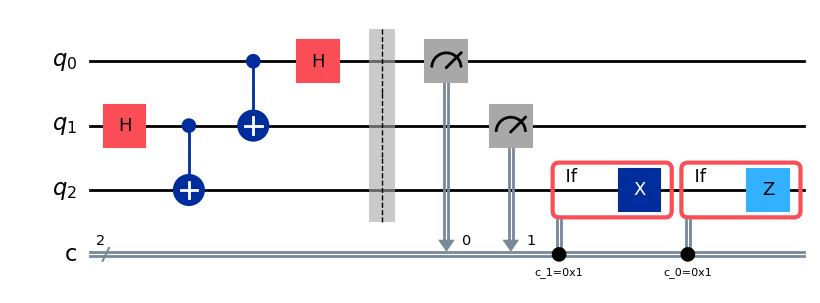
\includegraphics[width=0.45\textwidth]{Images/def_1.png}
  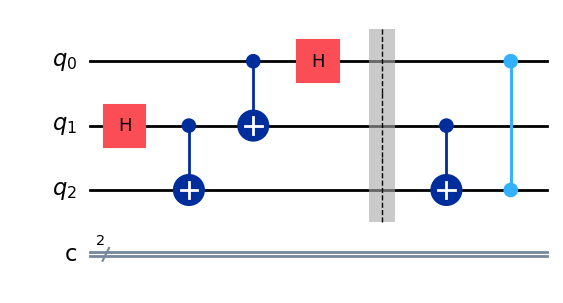
\includegraphics[width=0.45\textwidth]{Images/def_2.png}
  \caption{Deferred Measurement}
  \label{fig:deferred}
\end{figure}

\textbf{Motivation}: Most of the functionalities in quantum programming languages including \texttt{qiskit} and \texttt{cuda-quantum} ignore or support only minimal compiler optimizations for classically-controlled quantum operations. One may note that many such passes can avoided with good code and understanding of the quantum circuit. However, our proposed passes can improve scope of optimization by breaking the "measurement barrier". [\cite{branch}]

\subsection{Problem Statement}
The objectives of the project are as follows:
\begin{itemize}
  \item To study the existing transpiler passes in \texttt{qiskit} and their limitations in optimizing classically-controlled quantum operations.

  \item Given a quantum circuit with mid-circuit measurements and associated branches, we aim to optimize the circuit by integrating existing classical and quantum techniques. To this end, we explore three passes:
    \begin{itemize}
      \item Branch Merging \& Simplification
      \item If-Else Splitting \& Recombination 
      \item Hoare Optimizations across Measurements
    \end{itemize}

  \item We aim to investigate the viability of such passes and the compile time required to perform such passes.
\end{itemize}

%%%%%%%%%%%%%%%%%%%%%%%%%%%%%%%%%%%%%%%%%%%%%%%%%%%%%%%%%%%%%%%%%%%%%%%%%%%%

\section{Branch Merging \& Simplification}
A very common optimization on classical computations involves the merging of branches with similar predicates. For instance, consider the following code:
\begin{center}
\begin{BVerbatim}
  if (x == 0) {
      A;    //Statement 1
  }
  if (x == 0) {
      B;    //Statement 2
  }
\end{BVerbatim}
\end{center}

which can be simplified to:

\begin{center}
\begin{BVerbatim}
  if (x == 0) {
      A;    //Statement 1
      B;    //Statement 2
  }
\end{BVerbatim}
\end{center}

Similarly, we may choose to ignore branches when they have complementary predicates with same operations. This naturally extends to nested branches as well. Implementations and examples of these can be found in the code linked at the end of the document. The same idea can implemented to quantum circuits with mid-circuit measurements and associated branches. This may result in simplification/merging of certain branches, leading to more possible optimizations.

%%%%%%%%%%%%%%%%%%%%%%%%%%%%%%%%%%%%%%%%%%%%%%%%%%%%%%%%%%%%%%%%%%%%%%%%%%%%%

\section{If-Else Splitting \& Recombination}
The idea behind this pass follows directly from the classical branch prediction mechanisms. We would like to note the following differences:
\begin{itemize}
  \item All quantum gates (excluding measurements) are \emph{reversible}. In other words, one may easily revert operations on a qubit to its original state when necessary.
  \item Measurements are irreversible and generally do not commute with quantum gates. Hence, we cannot revert operations after measurements on measured qubits. This limits the scope of optimizations but can help with certain operations on unrelated qubits. We may choose to alleviate some of these constraints through other optimizations (later discussed).
  \item The optimization extent is dependent on several factors inclusing circuit area, nesting level of branching, window depth for optimization etc.
  \item Generalization is hard when each branch re-evaluates measured qubits. In such cases, one may be forced to split branches into dependent and non-dependent branches.
\end{itemize}

\begin{figure}[h]
\centering
  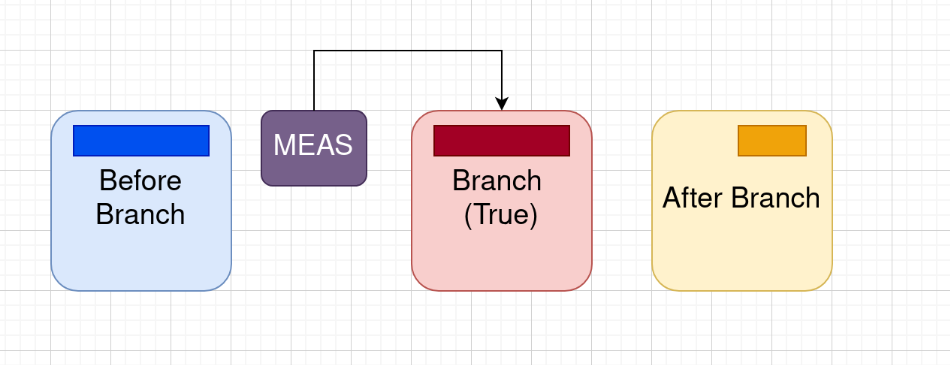
\includegraphics[width=0.45\textwidth]{Images/start.png}
  \caption{If-Else Circuit}
  \label{fig:ifelse}
\end{figure}

\begin{figure}[h]
\centering
  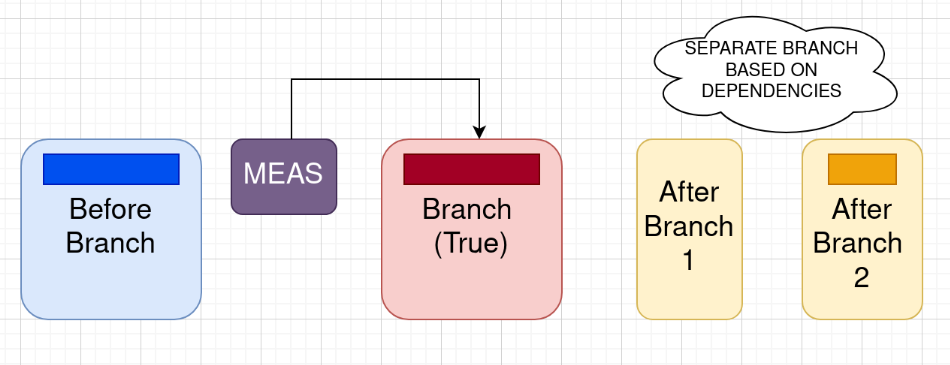
\includegraphics[width=0.45\textwidth]{Images/sep.png}
  \caption{Split Circuit}
  \label{fig:split}
\end{figure}

\begin{figure}[h]
\centering
  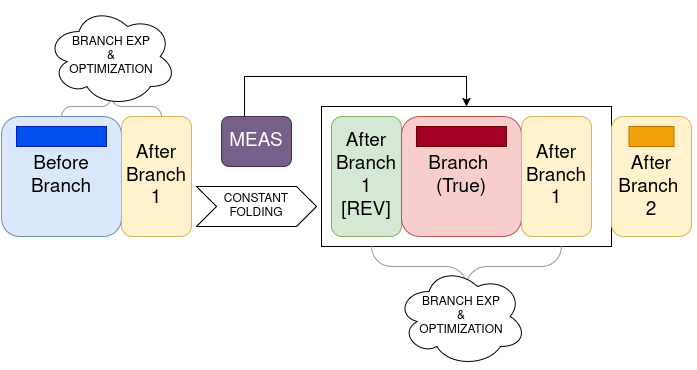
\includegraphics[width=0.45\textwidth]{Images/recomb.png}
  \caption{Recombined Circuit}
  \label{fig:recomb}
\end{figure}

\subsection{Phases}
The pass consists of the following phases with the circuit initially in a state like [\ref{fig:ifelse}]:
\begin{itemize}
  \item \textbf{Splitting}: Spilt the circuit after the branch into dependent and independent branches. We only work with the independent branches for optimization. [\ref{fig:split}]
  \item \textbf{Recombination}: Assuming the branch fails, we recombine before-branch with operations from after-branch (the indepedent branches). The \texttt{if-branch} is then replaced with a appropriate reversing and recombination. [\ref{fig:recomb}]
\end{itemize}

\subsection{Example \& Analysis}
Through manual implementations, we were able to see that for toy-examples, there is considerable reduction in gate-complexity. Note that we assume our basis-gate set \texttt{RZ, X, SX, CX} where \texttt{RZ} is a single-qubit rotation gate, \texttt{X} is a Pauli-X gate, \texttt{SX} is a square-root of X gate and \texttt{CX} is a controlled-X gate. The following example illustrates the optimization: [\ref{fig:toy}]\\

\begin{figure}[h]
\centering
  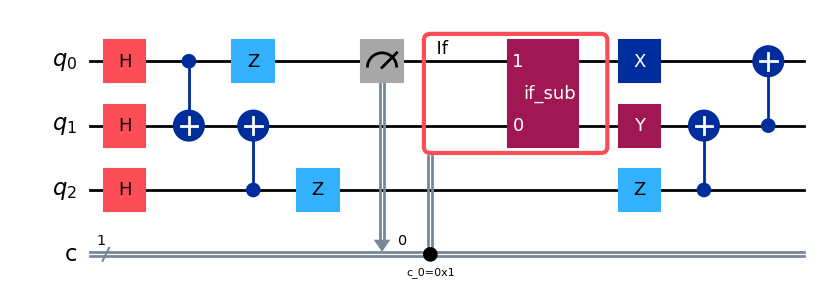
\includegraphics[width=0.45\textwidth]{Images/toy1.png}
  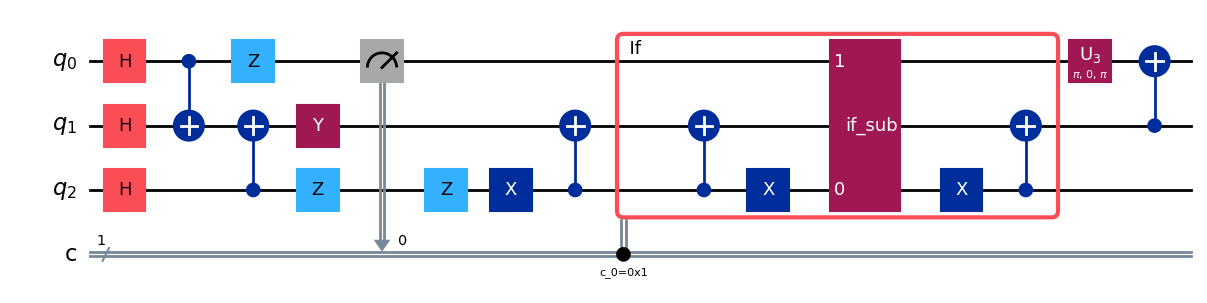
\includegraphics[width=0.55\textwidth]{Images/toy2.png}
  \caption{Toy Example for If-Else Splitting \& Recombination}
  \label{fig:toy}
\end{figure}

For utilitarian examples like quantum bit-flip error correcting codes, we observe very little improvement. Note that all these optimizations are highly dependent on other subcircuit structures.

\section{Hoare Optimizations across Measurements}
Hoare logic is a formal system used to reason about the correctness of computer programs. It provides a way to specify and prove properties of programs using preconditions and postconditions. Simply put, Hoare optimizations are a generalization of constant-folding. [\cite{hoare}] \\

In the context of quantum circuits, we can use Hoare logic to reason about the behavior of quantum operations and their interactions with classical control flow. Again these may be dependent on whether the initial state of qubits are known or not.

\subsection{Example}
A simple example of Hoare optimization is as follows [\ref{fig:hoare}]. Consider the circuit with the following operations:

\begin{figure}[h]
\centering
  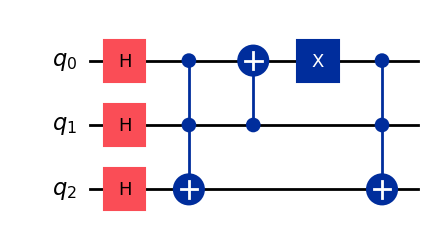
\includegraphics[width=0.45\textwidth]{Images/hoare_s1.png}
  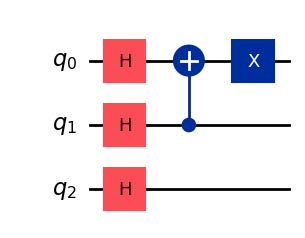
\includegraphics[width=0.30\textwidth]{Images/hoare_s2.png}
  \caption{Hoare Optimization Example}
  \label{fig:hoare}
\end{figure}

Consider the circuit [put label here] operating on three qubits $q_0, q_1, q_2$. After the Hadamard operations equally mix the states $q_0$ and $q_1$, we the \texttt{CX} operation transforms $(q_0, q_1) \xrightarrow{CX} (q_0 \oplus q_1, q_1)$. After another application of \texttt{X} on $q_0$, we have $(q_0 \oplus q_1, q_1) \xrightarrow{X} (q_0 \oplus q_1 \oplus 1, q_1)$. The two \texttt{CCX} operations are only activated when $q_0q_1 = 1$. After the transformation, we get $(q_0 \oplus q_1 \oplus 1)(q_1) = q_0q_1 \oplus q_1 \oplus q_1 = q_0q_1$. Thus, both \texttt{CCX} happen to work simultaneously and cancel out regardless.

\subsection{Types of Possible Optimizations}
\begin{itemize}
  \item \textbf{Across Measurements}: \texttt{qiskit} cannot optimize using Hoare logic when there are measurement-dependent operations sandwiched between target gates. One may simply check dependencies and appropriate ignore these operations. [\ref{fig:meas_12}] uses the same example quoted previously in [\ref{fig:hoare}] but with an additional branch sandwiched in.

  \item \textbf{On Measurements}: Similar to constant-folding, when we know the value of the measurement that determines other operations with certainty, we may simply remove the measurement and the branch. This will lead to standard optimizations. [\ref{fig:meas_34}] is an example where we can determine with certainty that the first qubit is in state $\ket{1}$ and upon measurement, the branch is executed all the time. We simply remove the measurement and the branch and cancel out circuits.

  \item \textbf{Internal Optimizations}: One may internally apply Hoare logic on branch subcircuits. This can be done with the knowledge of measured qubits as qubits take definite values after measurement. [\ref{fig:val_dep}] shows an example where we can implement the \emph{If-Else Splitting \& Recombination} pass in addition to the above Hoare optimization. 
\end{itemize}

\begin{figure}[h]
\centering
  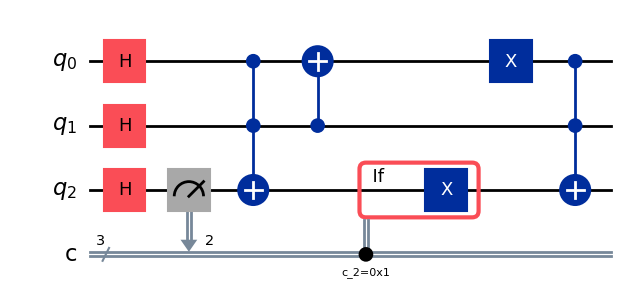
\includegraphics[width=0.45\textwidth]{Images/meas_1.png}
  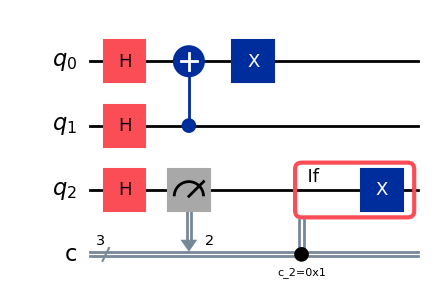
\includegraphics[width=0.30\textwidth]{Images/meas_2.png}
  \caption{Across Measurements}
  \label{fig:meas_12}
\end{figure}

\begin{figure}[h]
\centering
  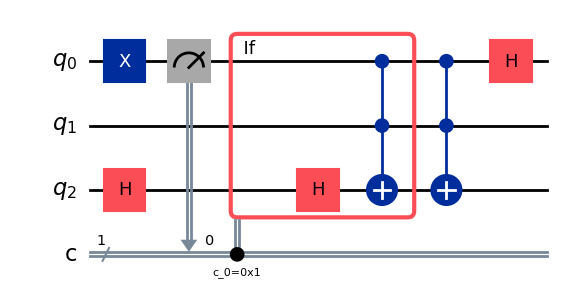
\includegraphics[width=0.45\textwidth]{Images/meas_3.png}
  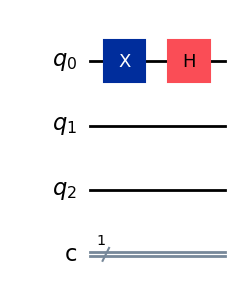
\includegraphics[width=0.20\textwidth]{Images/meas_4.png}
  \caption{On Measurements}
  \label{fig:meas_34}
\end{figure}

\begin{figure}[h]
\centering
  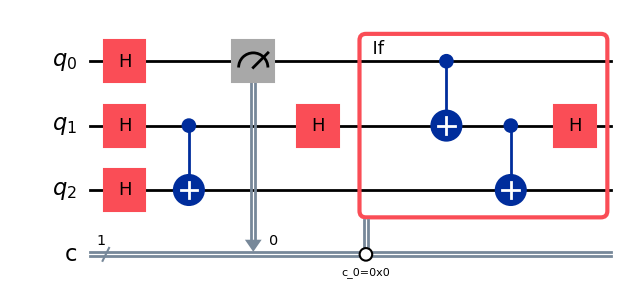
\includegraphics[width=0.45\textwidth]{Images/val_dep_1.png}
  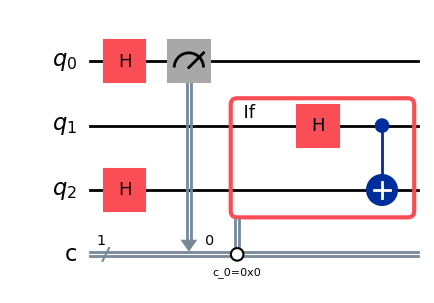
\includegraphics[width=0.30\textwidth]{Images/val_dep_2.png}
  \caption{Internal Optimizations}
  \label{fig:val_dep}
\end{figure}

\section{Conclusion \& Future Work}
We have included the proposed passes in [\href{https://github.com/kst164/CS5863-IPACO-Final-Project}{GitHub Link}]. Our future work will aim to generalize these passes and analyze performances on actual quantum devices. We also aim to explore the possibility of using these passes in other quantum programming languages like \texttt{cuda-quantum} [\cite{cudaq}] which exploit GPUs and TPUs to simulate quantum circuits.

\newpage
\bibliographystyle{aasjournal}
\bibliography{references}{}


\end{document}
